\de{ĐỀ THI HỌC KỲ II NĂM HỌC 2022-2023}{THPT Nguyễn Thượng Hiền}




%==Bài 1
\begin{bt}%[Dự án đề kiểm tra HKII NH22-23- Mui Doan]%[Nguyễn Thượng Hiền]%[0T7B2-1]
	Giải bất phương trình $x(x+5)\leq 2(x^2+2)$.
\loigiai{
Ta có $x(x+5)\leq 2(x^2+2)\Leftrightarrow x^2+5x\leq 2x^2+4\Leftrightarrow x^2-5x+4\geq 0$.\\
Cho $x^2-5x+4=0\Leftrightarrow\hoac{&x=1\\&x=4.}$\\
Bảng xét dấu
\begin{center}
	
\begin{tikzpicture}[font=\normalsize,t style/.style={style=solid}]
		\tkzTabInit[nocadre=false,lgt=2.5,espcl=2.5,deltacl=0.5]
		{$x$ /0.75, $x^2-5x+4$/0.75}
		{$ -\infty $,$ 1 $,$ 4 $,$ +\infty $}
		\tkzTabLine{  , +,0 , -,0  , +,  }  
	\end{tikzpicture}
\end{center}
Vậy tập nghiệm của bất phương trình là $S=(-\infty;1]\cup [4;+\infty)$.
}
\end{bt}
%==Bài 2
\begin{bt}%[Dự án đề kiểm tra HKII NH22-23- Mui Doan]%[Nguyễn Thượng Hiền]%[0T7B3-2]
	Giải phương trình $\sqrt{4x^2-x-1}+x-1=0$.
	\loigiai{
	Ta có 	$\sqrt{4x^2-x-1}+x-1=0\Leftrightarrow \sqrt{4x^2-x-1}=1-x$.\\
	Bình phương hai vế phương trình ta được
	\allowdisplaybreaks
	\begin{eqnarray*}
		&&4x^2-x-1=(1-x)^2
		\\
		&\Rightarrow&4x^2-x-1=1-2x+x^2
		\\
		&\Rightarrow&3x^2+x-2=0
		\\
		&\Rightarrow&\hoac{&x=-1\\&x=\dfrac{2}{3}.}
	\end{eqnarray*}
	Thử lại $x=-1$ và $x=\dfrac{2}{3}$ đều thỏa phương trình đã cho.\\
	Tập nghiệm của phương trình là $S=\left\{-1;\dfrac{2}{3}\right\}$.
	}
\end{bt}

%==Bài 3
\begin{bt}%[Dự án đề kiểm tra HKII NH22-23- Mui Doan]%[Nguyễn Thượng Hiền]%[0T8B1-2]
Trên giá sách có $4$ quyển sách Toán khác nhau, $5$ quyển sách Văn khác nhau và $6$ quyển sách Tiếng Anh khác nhau. Có bao nhiêu cách lấy $4$ quyển sách từ giá sách này sao cho có đủ ba môn và số quyển sách Toán nhiều nhất?
	\loigiai{
	 Chọn $1$ quyển Văn, $1$ quyển Tiếng Anh, $2$ quyển Toán\\
		Số cách chọn là $\mathrm{C}_5^1\cdot \mathrm{C}_6^1\cdot \mathrm{C}_4^2=180$ cách.
		}
\end{bt}

%==Bài 4
\begin{bt}%[Dự án đề kiểm tra HKII NH22-23- Mui Doan]%[Nguyễn Thượng Hiền]%[0T8B3-1]
Sử dụng công thức nhị thức Newton, khai triển biểu thức sau $(3-2x)^5$.	
	\loigiai{
	Ta có 	
	\begin{eqnarray*}
		(3-2x)^5&=&\mathrm{C}_5^0\,3^5+\mathrm{C}_5^1\, 3^4\cdot (-2x)^1+\mathrm{C}_5^2\, 3^3\cdot (-2x)^2+\mathrm{C}_5^3\, 3^2\cdot (-2x)^3+\mathrm{C}_5^4\, 3^1\cdot (-2x)^4+\mathrm{C}_5^5\, (-2x)^5
		\\
		&=&243-810x+1080x^2-720x^3+240x^4-32x^5.
	\end{eqnarray*}	
	}
\end{bt}
%==Bài 5
\begin{bt}%[Dự án đề kiểm tra HKII NH22-23- Mui Doan]%[Nguyễn Thượng Hiền]%[0T0G2-2]
	Trong cuộc thi nghiên cứu khoa học, một học sinh trường THPT Nguyễn Thượng Hiền thiết kế bảng điều khiển điện tử mở cửa phòng học của lớp mình. Bảng gồm $10$ nút, mỗi nút được ghi một số từ $0$ đến $9$ và không có hai nút nào được ghi cùng một số. Để mở cửa cần nhấn liên tiếp $3$ nút khác nhau sao cho theo thứ tự các lần bấm, tạo thành một số tự nhiên gồm $3$ chữ số khác nhau tăng dần (ví dụ $145$). Bạn An không biết quy tắc mở cửa trên, đã nhấn ngẫu nhiên liên tiếp $3$ nút khác nhau trên bảng điều khiển. Tính xác suất để An mở được cửa phòng học đó.
	\loigiai{
	Số phần tử của không gian mẫu là $n(\Omega)=10\cdot 9\cdot 8=720$.\\
	Gọi $A$	 là biến cố \lq\lq An mở được cửa phòng\rq\rq.\\
	Gọi $\overline{abc}$ là số tự nhiên có ba chữ số thỏa mãn $a<b<c$. Suy ra $a$; $b$; $c\neq 0$.\\
	Số cách chọn số tự nhiên $\overline{abc}$ thỏa mãn $a<b<c$ là một tổ hợp chập $3$ của $9$ phần tử $\{1;2;3;\ldots; 9\}$.\\
	Suy ra $n(A)=\mathrm{C}_9^3=84$.\\
	Vậy xác suất để An mở được cửa phòng là\\ $\mathrm{P}(A)=\dfrac{n(A)}{n(\Omega)}=\dfrac{84}{720}=\dfrac{7}{60}$.
	}
\end{bt}

\begin{bt}%[0T9B1-3]%[Dự án đề kiểm tra HKII NH22-23- Lê Hùng Thắng]%[THPT Nguyễn Thượng Hiền]%Câu 6
	Trong mặt phẳng $Oxy$, cho tam giác $ABC$ với $B(-2;5)$, $C(4;-10)$ và $G(-1;2)$ là trọng tâm tam giác $ABC$. Tìm tọa độ điểm $A$.
	\loigiai{
	Gọi $A(x;y)$, vì $G$ là trọng tâm của tam giác $ABC$ nên ta có
	\[\heva{&\dfrac{x+(-2)+4}{3}=-1 \\& \dfrac{y+5+(-10)}{3}=2} \Leftrightarrow \heva{&x=-5 \\&y=11.}\]\\
	Vậy $A(-5;11)$. 
	}
\end{bt}

\begin{bt}%[0T9B2-2]%[Dự án đề kiểm tra HKII NH22-23- Lê Hùng Thắng]%[THPT Nguyễn Thượng Hiền]%Câu 7
	Trong mặt phẳng $Oxy$, cho tam giác $ABC$ có $A(-1;5)$, $B(1;2)$ và $C(3; 4)$. Viết phương trình tổng quát của đường cao $BH$ và đường trung tuyến $AM$ của tam giác $ABC$.
	\loigiai{
	\begin{itemize}
\item Vì $BH$ qua $B(1;2)$ và có véc-tơ pháp tuyến là $\vec{AC}=(4;-1)$ nên $BH$ có phương trình là
\[4(x-1)-1(y-2)=0 \Leftrightarrow 4x-y-2=0. \]
\item $M$ là trung điểm $BC$ nên $M(2;3)$.\\
$AM$ có véc-tơ chỉ phương là $\vec{AM}=(3;-2)$.\\
Vì $AM$ qua $A(-1;5)$ và có véc-tơ pháp tuyến là $\vec{n}=(2;3)$ nên $AM$ có phương trình là
\[2(x+1)+3(y-5)=0 \Leftrightarrow 2x+3y-13=0.\]
	\end{itemize}

	}
\end{bt}

\begin{bt}%[0T9K3-6]%[Dự án đề kiểm tra HKII NH22-23- Lê Hùng Thắng]%[THPT Nguyễn Thượng Hiền]%Câu 8
\immini [thm]{Hình bên dưới mô phỏng một trạm thu phát sóng điện thoại di động đặt ở vị trí $I$ có toạ độ $(-2;1)$ trong mặt phẳng toạ độ (đơn vị trên hai trục là ki-lô-mét).
\begin{listEX}[1]
	\item Lập phương trình đường tròn mô tả ranh giới bên ngoài của vùng phủ sóng, biết rằng trạm thu phát sóng đó được thiết kế với bán kính phủ sóng $3$ km.
	\item Tính theo đường chim bay, xác định khoảng cách ngắn nhất để một người ở vị trí $B$ có toạ độ $(-3;4)$ di chuyển được tới vùng phủ sóng theo đơn vị ki-lô-mét.
\end{listEX}
}
{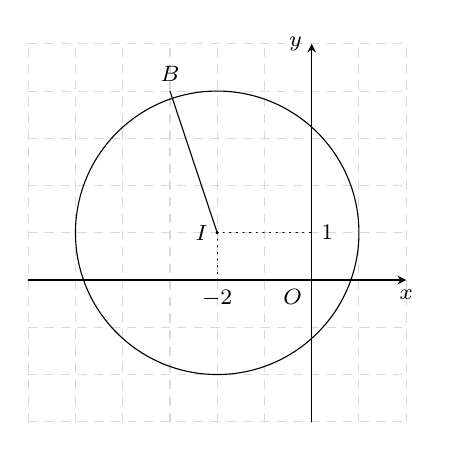
\begin{tikzpicture}[scale=0.6,>=stealth, font=\footnotesize, line join=round, line cap=round]
		\def\xmin{-6} \def\xmax{2}
		\def\ymin{-3} \def\ymax{5}
		\draw[color=gray!30,dashed] (\xmin,\ymin) grid (\xmax,\ymax);
		\draw[->] (\xmin,0)--(\xmax,0) node [below]{$x$};
		\draw[->] (0,\ymin)--(0,\ymax) node [left]{$y$};
		\node at (0,0) [below left]{$O$};
		\clip (\xmin+0.1,\ymin+0.1) rectangle (\xmax-0.1,\ymax-0.1);
		\draw (-2,1)node [left] {$I$} circle (3) (-3,4)node [above] {$B$}--(-2,1);
		\draw[dotted](-2,0) node [below] {$-2$}|-(0,1) node [right]{$1$};
		\fill (-2,1) circle (1pt) 
		(-2,1) circle (1pt);
	\end{tikzpicture}
}
	\loigiai{
	\begin{listEX}[1]
	\item Đường tròn mô tả ranh giới có tâm là $I(-2;1)$ và có bán kính $R=3$ nên phương trình của đường tròn là $(x+2)^2+(y-1)^2=9$.
	\item Ta có $\vec{BI}=(1;-3) \Rightarrow BI=\sqrt{10}>3=R$.\\
	Từ vị trí $B$ để đường đi đến vùng phủ sóng ngắn nhất thì phải đi theo hướng $\vec{BI}$.\\
	Quãng đường đi ngắn nhất là $d=BI-R=\sqrt{10}-3 \approx 0{,}162$ km.	
	\end{listEX}	
	}
\end{bt}

\begin{bt}%[0T9T4-0]%[Dự án đề kiểm tra HKII NH22-23- Lê Hùng Thắng]%[THPT Nguyễn Thượng Hiền]%Câu 9
\immini [thm]{	Mặt Trăng là một vệ tinh tự nhiên của Trái Đất, chuyển động quanh Trái Đất theo quỹ đạo là một đường elip với tâm Trái Đất là một tiêu điểm. Độ dài trục lớn, độ dài trục nhỏ của quỹ đạo lần lượt là $768800$ km và $767640$ km. Chọn hệ tọa độ thích hợp và viết phương trình chính tắc của elip nói trên.
}
{\begin{tikzpicture}[scale=0.5,>=stealth, font=\footnotesize, line join=round, line cap=round]
		\def\xmin{-4} \def\xmax{4}
		\def\ymin{-3} \def\ymax{3}
		%		\draw[color=gray!30,dashed] (\xmin,\ymin) grid (\xmax,\ymax);
		\draw[<->] (\xmin,0)--(\xmax,0);% node [below]{$x$};
		\draw[<->] (0,\ymin)--(0,\ymax);% node [left]{$y$};
		%		\node at (0,0) [below right]{$O$};
%		\clip (\xmin+0.1,\ymin+0.1) rectangle (\xmax-0.1,\ymax-0.1);
		\draw (0,0) ellipse (4cm and 3cm);
		\fill [gray] (-1,0) circle (8pt);
		\fill [gray] (60:4cm and 3cm) circle (5pt);
		\path (-1,0) node [above left]{Trái đất} 
		(1.8,1) node [above,rotate=-30]{Mặt trăng};
	\end{tikzpicture}
}
	\loigiai{
\immini{Chọn gốc tọa độ là giao điểm của hai trục elip.\\
Theo đề bài $\heva{&2a=768800 \\&2b=767600}  \Rightarrow \heva{&a=384400 \\&b=383800.}$\\
Phương trình của elip là $\dfrac{x^2}{384400^2}+\dfrac{y^2}{383800^2}=1$.
	}
{\begin{tikzpicture}[scale=0.5,>=stealth, font=\footnotesize, line join=round, line cap=round]
		\def\xmin{-5} \def\xmax{5}
		\def\ymin{-4} \def\ymax{4}
		%		\draw[color=gray!30,dashed] (\xmin,\ymin) grid (\xmax,\ymax);
		\draw[->] (\xmin,0)--(\xmax,0) node [below]{$x$};
		\draw[->] (0,\ymin)--(0,\ymax) node [left]{$y$};
		\node at (0,0) [below right]{$O$};
		\clip (\xmin+0.1,\ymin+0.1) rectangle (\xmax-0.1,\ymax-0.1);
		\draw (0,0) ellipse (4cm and 3cm);
		\fill [gray] (-1,0) circle (8pt);
		\fill [gray] (60:4cm and 3cm) circle (5pt);
		\path (-1,0) node [above left]{Trái đất} 
		(60:4cm and 3cm) node [above]{Mặt trăng};
	\end{tikzpicture}
}
}
\end{bt}

\begin{bt}%[0T7T3-2]%[Dự án đề kiểm tra HKII NH22-23- Lê Hùng Thắng]%[THPT Nguyễn Thượng Hiền]%Câu 10
\immini [thm]{	Hòn đảo $D$ cách bờ một khoảng $CD=4$ km. Ngôi làng $B$ cách $C$ một khoảng $7$ km. Nhà nước muốn xây dựng một trạm y tế trên đất liền, sao cho có thể phục vụ được cho dân cư ở cả đảo $D$ và làng $B$. Biết trung bình vận tốc di chuyển tàu cứu thương là $100$ km/h, xe cứu thương là $80$ km/h. Vậy nên đặt trạm y tế cách đảo $D$ bao xa để thời gian cứu thương cho hai địa điểm là như nhau?
}
{\begin{tikzpicture}[scale=0.6,>=stealth, font=\footnotesize, line join=round, line cap=round]
		\path (0,0) coordinate (C)
		(4,0) coordinate (A)
		(7,0) coordinate (B)
		(0,4) coordinate (D);
		\draw (C)--(D) node[above,sloped,pos=0.5]{$4$ km};
%		\draw (C)--(A) node[below,sloped,pos=0.5]{$x$ km};
		\draw (B)--(C) (A)--(D);
		\draw [<->] ($(B)+(0,-0.8)$)--($(C)+(0,-0.8)$) node[below,sloped,pos=0.5]{$7$ km};
		\fill [gray] (A) circle (5pt) 
		(B) circle (5pt)
		(C) circle (3pt) 
		(D) circle (5pt);
		\path (A) node [below]{$A$} 
		(B) node [below]{$B$}
		(C) node [below]{$C$}
		(D) node [left]{$D$};
	\end{tikzpicture}
}
	\loigiai{
\immini{Đặt $AC=x$ (km) với $x>0$, khi đó $AB=7-x$ và $AD=\sqrt{16+x^2}$.\\
Thời gian đi từ $D$ đến $A$ là $t_1=\dfrac{\sqrt{16+x^2}}{100}$.\\
Thời gian đi từ $B$ đến $A$ là $t_2=\dfrac{7-x}{80}$.\\
Để thời gian cứu thương cho hai địa điểm như nhau, ta có
\[t_1=t_2 \Leftrightarrow \dfrac{\sqrt{16+x^2}}{100} = \dfrac{7-x}{80}.\] 	
}
{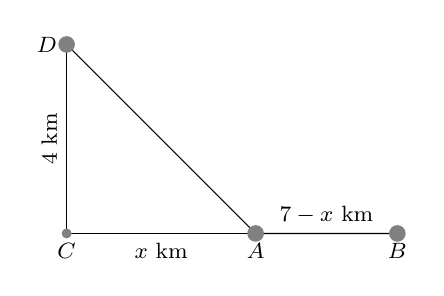
\begin{tikzpicture}[scale=0.6,>=stealth, font=\footnotesize, line join=round, line cap=round]
		\path (0,0) coordinate (C)
		(4,0) coordinate (A)
		(7,0) coordinate (B)
		(0,4) coordinate (D);
		\draw (C)--(D) node[above,sloped,pos=0.5]{$4$ km};
		\draw (C)--(A) node[below,sloped,pos=0.5]{$x$ km};
		\draw (A)--(B) node[above,sloped,pos=0.5]{$7-x$ km} (A)--(D);
		\fill [gray] (A) circle (5pt) 
		(B) circle (5pt)
		(C) circle (3pt) 
		(D) circle (5pt);
		\path (A) node [below]{$A$} 
		(B) node [below]{$B$}
		(C) node [below]{$C$}
		(D) node [left]{$D$};
\end{tikzpicture}
}
\noindent Giải phương trình ta được nghiệm $x=3$.\\
Vậy khoảng cách từ đảo đến trạm y tế là $AD=5$ km.
	}
\end{bt}


